\documentclass[letterpaper,12pt]{article}
\usepackage[utf8]{inputenc}
\usepackage{booktabs}
\usepackage{tabularx}
\usepackage{makecell}
\usepackage{graphicx}
\usepackage{svg}

\graphicspath{{./figs/}}
\def\svgwidth{\textwidth}


\renewcommand{\theadalign}{bl}
\renewcommand\theadfont{\bfseries}

\newcommand{\itwoc}{I\textsuperscript{2}C}


%opening
\title{Modular Electric Skateboard}
\author{Nick Fajardo, Phillip Konyeaso, Zane Weissman}

\begin{document}

\maketitle

\begin{abstract}
The Modular Electric Skateboard (MESB) is an electric skateboard (ESB) that allows the user to mix and match components tailored to a specific user’s needs. The MESB is equipped with a TBD watt motor controlled by a handheld RC controller and capable of acheiving speeds as high as TBD. The deck, the part of the board on which the user stands while riding, can be disassembled and reassembled by hand to swap out major mechanical components of the board. The board's electrical system includes rails for mounting hot-swappable accessories.

\end{abstract}

\section{Background}
In order to commute from one place to another in an urban environment, one has to consider multiple options in order to get around without a significant time delay in their route. Solutions exist, such as bicycles, busses, and trains. However, as of recently, there has been a growing market in a specific solution, electric skateboards. In order to understand this market, one should be knowledgeable on skateboard parts, electric skateboard parts, and available ESBs for consumers.
\subsection{Skateboard Parts and Terminology}
Skateboarding has been around since the mid 1900’s, and has changed drastically since its introduction. The diagrams on the right below show the different parts that make a modern complete skateboard, and the list below defines each part in detail.
\begin{itemize}
\item Griptape - Main method of retaining a surface that has plenty of friction between the rider and the skateboard. Comes in different grits (measure of “roughness”) and colors
\item Deck - The plate where the trucks and griptape is attached. It is essential for any deck to be reliable, but also have some amount of flex for comfort. Varies in size and material.
\begin{itemize}
\item Nose - Front of the board. A typical skateboard has a nose that is angled up
\item Tail - rear of the board. A typical skateboard has a tail that is angled up
\end{itemize}
\item Trucks - The assembly that holds all the parts needed to have non powered, fixed wheels below the deck.
\begin{itemize}
\item Riser Pad - pad used to add distance between the wheel and the deck. Often made of a material conducive to dampening vibration, such as rubber or cork.
\item Base Plate - metal piece used for the rest of the truck assembly to be attached to. Has a threaded rod sticking out of it for the assembly to align and attach to.
\item Bushings - Spacers between the Kingpin, the hanger, and the base plate. Bushings are used to adjust the force required to turn while riding. I.E., a harder to compress bushing will require the user to lean to a direction more in order to perform the same degree of turn as a softer to compress bushing. Often made of some sort of rubber polymer
\item Kingpin - Nut used to cap the hanger and bushing assembly. Most often a locknut.
\item Axel (and Axle Nut) - rod used to attach the wheels.
\item Bearings - device inserted into the wheels in order for the wheels to rotate smoothly
\item Wheels - device that allows the skateboard to move, varies in size, shape, and color.
\end{itemize}
\item Hardware - term for the nuts and bolts needed to attach the base plate to the deck.
\item Longboard - Type of skateboard often used for traveling long distances. Has an elongated deck and often is more flexible than a skateboard.
\end{itemize}

\subsection{Electric Skateboards}
Electric Skateboards are a variant of skateboards that attach a motor and gearing system to either the back and/or front of the board. Most ESBs on the market today are tailored to provide a device that can handle a moderate commute, while being lite and portable. Hence, most often than not adopting a longboard and adding a drive system that consists of motors with a battery. 
One example of an ESB is the Boosted Board brand “Dual+ XR” pictured on the right, which happens to also be one of the most popular off the shelf ESBs on the market today. It retails for \$1,599 and claims a top speed of 22 mph and a range of 14 miles with its 2000W motor and regenerative braking. Some more examples of popular ESBs can be found in the table below:\\\ \\
\resizebox{\textwidth}{!}{
\begin{tabular}{>{\bfseries}l l l l l}
Board Name & Top Speed (mph) & Battery Range (Miles) & Weight (lbs) & Price (Dollars) \\\hline
Inboard M1 & 22 & 7 & 14.5 & 1,000 \\
Boosted Plus/Stealth & 22/24 & 14 & 17 & 1,399/1.599 \\
Blink Qu4tro & 23 & 22 & 24 & 1,699 \\
Boosted Mini S/X & 18/20 & 7/14 & 15/16.8 & 749/999 \\
Onewheel +/+XR & 19 & 5-7/12-18 & 25 & 1,399/1,799 \\
\end{tabular}
}

\section{System Overview} 
The modular electric skateboard is an electric skateboard with a deck comprised of multiple sections which can be interchanged and replaced, a handheld remote controller for controlling the electric motor, a rail/data bus system attached to the underside of the deck which is capable of housing a number of accessories, and a small computer system which manages those accessories via a simple but flexible API.

\subsection{Mechanical Systems}
\subsection{Control Systems and Control Processing}

%\includesvg[width=\textwidth]{rt}
%\input{figs/rt.pdf_tex}
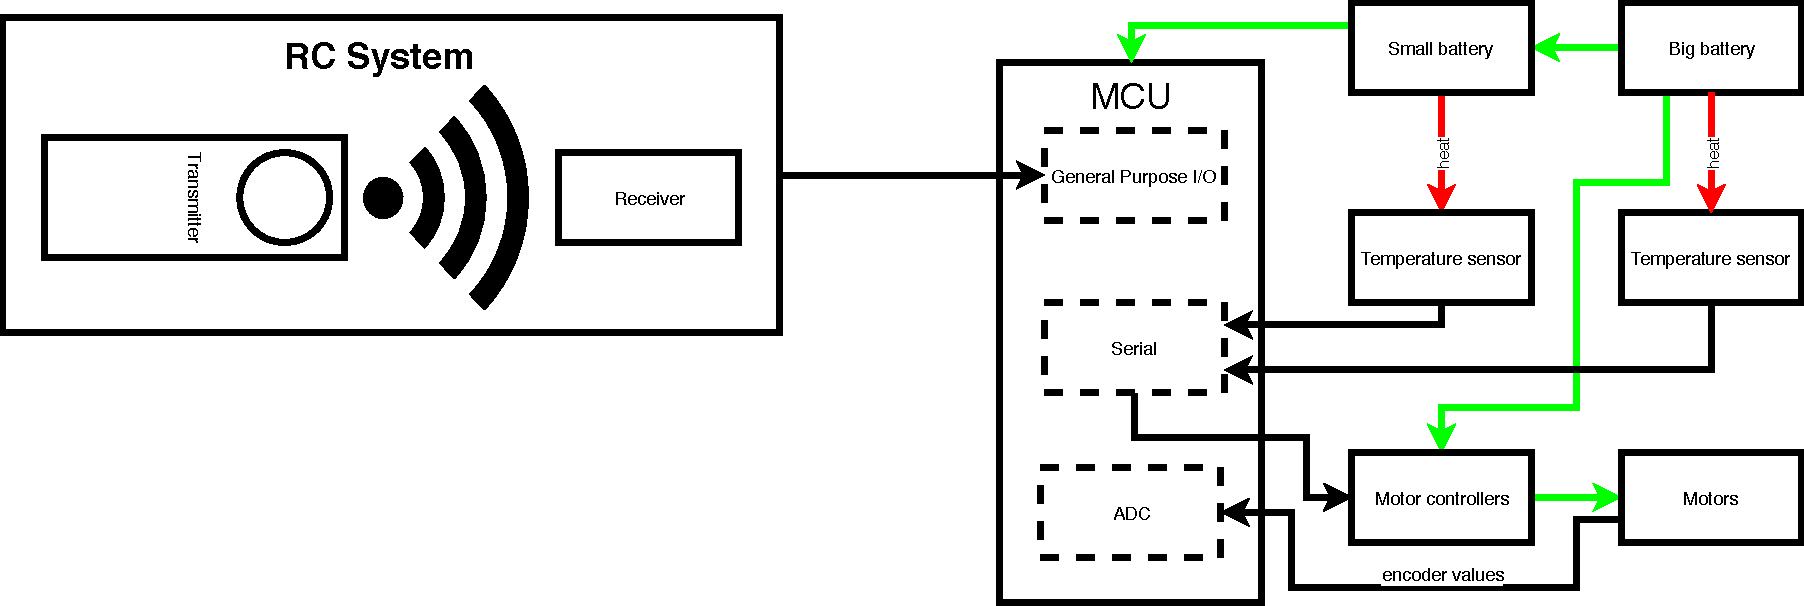
\includegraphics[width=\linewidth]{rt.pdf}
\subsection{Electrical and Power Systems}
\subsection{Computer and Accessory System}

\section{Design Analysis}
\subsection{Trade Studies}
This section breaks down in detail several tradeoffs of components, protocols, etc. which had to be considered once the system level design was finished. Each column compares the qualities of a certain attribute of the systems under study, and lists the point value score assigned to each quality. The maximum acheivable score in each category is listed in the header of each category with a ``/'' preceding it; the maximum acheivable total score is listed in the header of the leftmost column listing the names of the systems being compared.

\subsubsection{Real Time Microcontroller}
Before choosing a specific processor or development board, several microcontroller (MCU) platforms were compared. At least some variants of each of these microcontrollers would meet the basic requirements of the MCU for the real time control system on the MESB, such as hardware interrupts and an appropriate number of analog to digital converters, timers, etc.:
\\\ \\
\resizebox{\textwidth}{!}{
\begin{tabular}{>{\bfseries}l>{\bfseries}r lr lr lr lr lr}
\toprule
%platform & Total Points & Price & Points (5) & architecture & Points (4) & clock & Points (2) & current draw & Points (2) & Familiarity/ease of use & Points (6)
%\tradecat{Platform} & \tradecat{Price} \\
\thead{Platform} & /20 & \thead{Price} & /5 & \thead{Architecture} & /5 & \thead{Core \\ Clock} & /2 & \thead{Current \\ Draw } & /2 & \thead{Familiarity \\ \& Ease of Use} & /6\\
\cmidrule(r){1-2} \cmidrule(r){3-4} \cmidrule(r){5-6} \cmidrule(r){7-8} \cmidrule(r){9-10} \cmidrule(r){11-12}
%Name & Total Points & Price & Points\\
MSP430 & 16 & \$10-18 & 4 & 16 bit RISC & 3 & 8-24 MHz & 1 & ~5 mA & 2 & High & 6\\
STM32 Cortex & 13 & \$10-25 & 4 & 32 bit ARM Cortex-m & 4 & 32-400MHz & 2 & ~100-500 uA/MHz & 0 & Moderate & 3\\
ATMega328P & 15 & \$3-10 & 5 & 8 bit AVR RISC & 1 & up to 20 MHz & 1 & ~5 mA & 2 & High & 6\\
\bottomrule
\end{tabular}
}
\\\ \\
Though all of these platforms had their advantages and disadvantages, the MSP430 was chosen for its capable and flexible 16-bit architecture, its low cost and power consumption, and for the developers' familiarity with the ins and outs of its hardware and firmware.

The next table compares various MSP430 development boards. The names are truncated to avoid redundancy and save space; the development boards being compared are the MSP-EXP430FR2355, MSP-EXP430FR2433, etc., using the MSP430FR2355, MSP430FR2433, etc. microprocessors, respectively.\\
\\
\resizebox{\textwidth}{!}{
\begin{tabular}{>{\bfseries}l>{\bfseries}r lr lr lr lr lr}
\toprule
\thead{MCU} & /15 & \thead{Price}& /8 & \thead{Core Clock} & /2 & \thead{RAM + \\ Storage} & /5 & \thead{Current Draw} & /3 & \thead{ADCs} & /2 \\
\cmidrule(r){1-2} \cmidrule(r){3-4} \cmidrule(r){5-6} \cmidrule(r){7-8} \cmidrule(r){9-10} \cmidrule(r){11-12}
FR2355 & 12 & \$13 & 5 & 24 MHz & 2 & 32KB & 2 & 142 uA/MHz,{\raise.5ex\hbox{$\scriptstyle\sim$}}1 uA standby & 1 & 1x12b & 2\\
FR2433 & 13 & \$10 & 8 & 16 MHz & 1 & 15.5KB & 1 & 125 uA/MHz; $<$1 uA standby & 2 &8x10b & 1\\
FR5994 & 11 & \$17 & 1 & 16 MHz & 1 & 264KB & 5 & 118 uA/MHz; 500 nA standby & 2 & 1x12b & 2\\
FR4133 & 10 & \$14 & 4 & 16 MHz & 1 & 15.5KB & 2 & 126 uA/MHz; $<$1 uA standby & 2 &10x10b &1\\
FR6989 & 10 & \$18 & 0 & 16 MHz & 1 & 128KB & 4 & 100 uA/MHz; 350 nA standby & 3 & 16x12b & 2\\
FR5969 & 11 & \$16 & 2 & 16 MHz & 1 & 62KB & 3 & 100 uA/MHz; .4 uA standby & 3 & 16x12b & 2\\
F5529 & 16 & \$13 & 5 & 25 MHz & 2 & 136KB & 4 & 150 uA/MHz; 2 uA standby & 3 & 1x12b & 2\\
\bottomrule
\end{tabular}
}
\\\ \\
The MSP430F5529 offers above average MSP430 performance for below average price. While its higher clock rate may not be necessary, 128KB of flash memory provide a comfortable amount of program storage space
\subsubsection{Accessory Bus Serial Protocol}
The following table compares several serial protocols which were considered for the main accessory bus:\\
\resizebox{\textwidth}{!}{
\begin{tabular}{>{\bfseries}l>{\bfseries}r lr lr lr lr }
\toprule
\thead{Name} & /27 & \thead{Wires, \\ Shared} & /3 & \thead{Add'l Wires \\ per Device }& /10 & \thead{Speed} & /4 & \thead{Ease\\ of Use} & /10\\
\cmidrule(r){1-2} \cmidrule(r){3-4} \cmidrule(r){5-6} \cmidrule(r){7-8} \cmidrule(r){9-10} 
\itwoc & 25 & 2 & 2 & 0 & 10 & 100k-3.4Mbps & 3 & easy & 10\\
CAN & 17 & 2 & 2 & 0 & 10 & 1Mbps & 3 & hard & 2\\
SPI & 15 & 3 & 1 & 1 & 3 & 10Mbps & 4 & medium & 7\\
UART & 15 & 0 & 3 & 2 & 0 & {\raise.5ex\hbox{$\scriptstyle\sim$}}10-100kbps & 2 & easy  & 10\\
LIN & 17 & 1 & 3 & 0 & 10 & 20kbps & 1 & hard & 3\\
\bottomrule
\end{tabular}
}\\\ \\
\itwoc{} was chosen for its two-wire communication, ease of use, and more than sufficient speed. Some other serial protocols shared some but not all of these desirable attributes, but \itwoc{} scored nearly perfectly overall.
\end{document}
